\documentclass[main.tex]{subfile}

\begin{document}

\section{Why This Seminar?} 
\label{sec:why_this_seminar_}
\begin{frame}{Why this Seminar?}
	\begin{itemize}
		\item Review C Programming Concepts
		\item Prepare you for the microcontroller lab
		\item Help!
	\end{itemize}
\end{frame}

\begin{frame}{Live Demo}
	\begin{itemize}
		\item Use Windows Visual Studio to follow along!
		\item \emph{Note: I'm not using Win VS ... I'm on Linux!}
		\item \textbf{Please play around and break things!}
	\end{itemize}
\end{frame}

\begin{frame}{Plan of Action}
	\begin{itemize}
		\item Research: The math of the problem.
		\item Plan: From idea to program - prewriting
		\item Execute: write and test the program
	\end{itemize}
\end{frame}

\section{Prewriting} 
\label{sec:prewriting}

\begin{frame}[fragile]{Example Problem - Pumpkin Launch}
	\begin{itemize}
		\item Let's make a device to help us calculate the max distance and height
				our pumpkin will travel
		\item Depends on the launch angle: 
			\[ 
				\vec{r_o} = \vec{0} , 
				\vec{v_{o}} = 
					\begin{bmatrix} \cos{\theta} \\ \sin{\theta} \end{bmatrix} 
			\]
		\item Max height: 
			\[
				\begin{bmatrix}
					   0 & \frac{v_{o_{x}}}{g}
					\\ 0 & \frac{v_{o_{y}}}{2 g}
				\end{bmatrix}\vec{v_0}
			\]
		\item Max distance: \[d = \frac{2 v_{o_{x}} v_{o_{y}}}{g}\]
	\end{itemize}
	
	% subsection pumpkin_launch_ (end)
\end{frame}

\begin{frame}{Prewriting}
	\begin{itemize}
		\item Plan how you'll go from math to code: psuedocode
		\item Write out algorithms.
		\item Develop program execution sequence.
	\end{itemize}
\end{frame}

\begin{frame}[fragile]{Prewriting: Psuedocode}
	\begin{itemize}
		\item Use block Diagrams: 
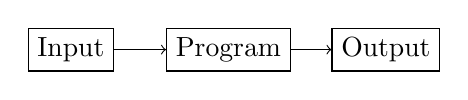
\begin{tikzpicture}
	\node[draw,rectangle] (in) at (0,0) {Input};
	\node[draw,rectangle] (prog) at (2,0) {Program};
	\node[draw,rectangle] (out) at (4,0) {Output};

	\draw[->] (in) -- (prog);
	\draw[->] (prog) -- (out);
\end{tikzpicture}

		\item Use psuedocode: 
			\begin{algorithmic}
				\STATE $S \leftarrow \text{Get INPUT}$
				\STATE $\text{OUTPUT} \leftarrow \text{Program } S$
				\RETURN OUTPUT
			\end{algorithmic}

	\end{itemize}
\end{frame}

\begin{frame}
	
	Now that we're ready to write the program how do we get tell the computer what
	we want?

	\begin{itemize}
		\item Variables
			\begin{itemize}
				\item Regular Variables
				\item Arrays
			\end{itemize}
		\item Functions
		\item Control Statements
	\end{itemize}

\end{frame}


\begin{frame}{Hello World}
	Let's start with a hello world program. See \textit{helloWorld.c}
	\begin{itemize}
		\item What's the main thing?
		\item Printf: short for ``print formated string''
	\end{itemize}
\end{frame}

% section prewriting (end)

% section why_this_seminar_ (end)

\section{Programing Basics} 
\label{sec:programing_basics}

\section{Variables}
\label{sec:variables_scope_and_arrays}

\begin{frame}[fragile]{Variables - a Review}
	\begin{itemize}
		\item Containers for memory - why do we use variables in math?
		\item Types: What kind of data am I using?
		\item Syntax:
			\begin{lstlisting}
//a declaration
<type> <name>; 

//an instanciation 
// (which means "instance creation")
<name> = <value>;

//both at the same time
<type> <name>  = <value>;
			\end{lstlisting}
		\item Let's see an exmple - to the example cave!
	\end{itemize}
\end{frame}

% section variables (end)

\section{Functions} 
\label{sec:functions}

\begin{frame}
	\begin{itemize}
		\item Functions are used to modularize code
		\item Variables must be initialized at the top of the function.
	\end{itemize}
\end{frame}

\begin{frame}[fragile]
	\begin{itemize}
		\item Function in math: $\text{name}(\text{args}) = \text{stuff}$
		\item Example: $foo(x,y) = x+y$
		\item Some basic function syntax:
	\begin{lstlisting}
<type> name(<args>)
{

}
	\end{lstlisting}
	\item Exmaple: 
		\begin{lstlisting}
double foo(double x, double y)
{
	return x+y;
}
		\end{lstlisting}
	\end{itemize}
\end{frame}

\begin{frame}[fragile]{Functions and Scope}
Scope decides which variable to use when its used within some piece of code.

	\begin{lstlisting}[language=c]

int x = 0;

int f(int x)
{
	//which x is being used to calculate 
	//the result of this function?
	return (x+2);
}

int main(char argc, char** argv)
{
	int x = 0;
}

	\end{lstlisting}
\end{frame}

% section functions (end)

\section{Arrays}
\label{sec:arrays}

\begin{frame}[fragile]{Arrays}
	\begin{itemize}
		\item How can we store tables or lists of data? (pretend arrays didn't exist
			yet)
		\item Arrays - how we represent sets of data.
		\item Syntax:
			\begin{lstlisting}
<type> <name> [<size>];

<name>[<index>] = <value>;
			\end{lstlisting}
		\item why do indeces begin at 0?
	\end{itemize}
\end{frame}

\begin{frame}[fragile]{Practical Use of Arrays}
	Calculating max height: see: \textit{arrays.c}
\end{frame}

% section arrays (end)


\section{Compiling} 
\label{sec:compiling}

% section compiling (end)

\section{Debugging} 
\label{sec:debugging}

\begin{frame}{When Something Goes Wrong Blame:}

	\begin{itemize}
			\only<1->{\item The end user!}
			\only<2->{\item The programmer (you)!}
			\only<3->{\item The other programmer!}
	\end{itemize}

\end{frame}

% section debugging (end)

\section{Tips and Tricks} 
\label{sec:tips_and_tricks}

\begin{frame}{Tips and Tricks}
	Generalize when Possible.

	TODO: add example here.
\end{frame}

% section tips_and_tricks (end)

\end{document}
